% Author: Matthew Turner

\documentclass[11pt,letterpaper]{article}
% \documentclass[11pt]{report}
% \documentclass{report}
% \documentclass{book}
\usepackage[bookmarks]{hyperref}
\usepackage{amssymb,amsmath}
% \usepackage{fullpage}
\usepackage{tabulary}
\usepackage{tabularx}

% \usepackage[margin=1.00in]{geometry}
\usepackage[margin=0.90in]{geometry}
\usepackage{float}

\usepackage{caption}
\usepackage{booktabs}
\usepackage{pslatex}
\usepackage{apacite}
\usepackage{subcaption}
\usepackage{pgfplots}
\usepackage{wrapfig}
\usepackage[english]{babel}
\usepackage{lmodern}
\usepackage{setspace}
\doublespace
% \usepackage{url}
\usepackage{bigfoot}
\usepackage[export]{adjustbox}
\setlength\intextsep{0pt}

\usepackage{graphicx}

\title{Identity signaling model progress}

\author{} %{Matthew A.~Turner}}

\begin{document}
\maketitle

\section*{Preliminary results}

For these preliminary results I focus on the evolution of signaling strategies,
and set receiving strategies to be randomly assigned with probability 0.5 to
each agent at model initialization. I set $R=0.5$, $s=0.25$, $d=\delta=0.25$,
and $N=100$. After signaling, agents go through 10 rounds of assortment/interaction,
followed by evolution after the 10 rounds of interaction. The model has been
run out to 100 timesteps where timeseries are nearly stable, though we will
want more timesteps for our final study, or perhaps adjust the number of 
assortment/interaction rounds up or down per timestep, to guarantee full 
stability (see Figure~\ref{fig:exampleSeries}).

\subsection*{Density of covert signalers vs. $r/R$ and homophily, $w$}

Based on results from ``Evolution of covert signaling'' (``ECS''), I designed
the first agent-based model experiment to determine the dependence of the
density of covert signalers in the population ($\rho_C$) on
the receptiveness of the population to covert signals ($r$) and the
importance of homophily ($w$) to assortment. 

I systematically varied $r/R$ by setting $R=0.5$ and varied 
$r \in \{0.0, 0.05, 0.1, \ldots, 0.45\}$ to get $r/R \in \{0.0, 0.1, \ldots, 0.9\}$.
I varied homophily similartly to $r$, $w \in \{0.0, 0.5, \ldots, 0.45\}$. Note
that both $r$ and $w$ are bounded above by 0.5.


\begin{figure}[H]
  \centering
  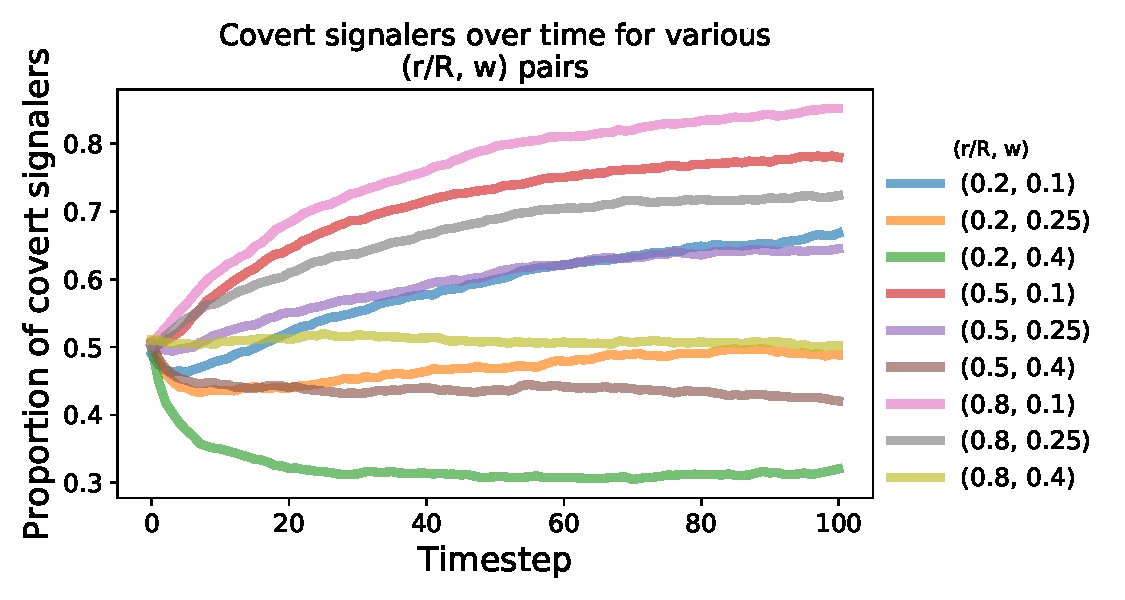
\includegraphics[width=0.8\textwidth]{Figures/exampleMidrangeSeries.pdf}
  \caption{Timeseries of nine combinations of $r/R$ and $w$.}
  \label{fig:receptivityHomophilySeries}
\end{figure}


\begin{figure}[H]
  \centering
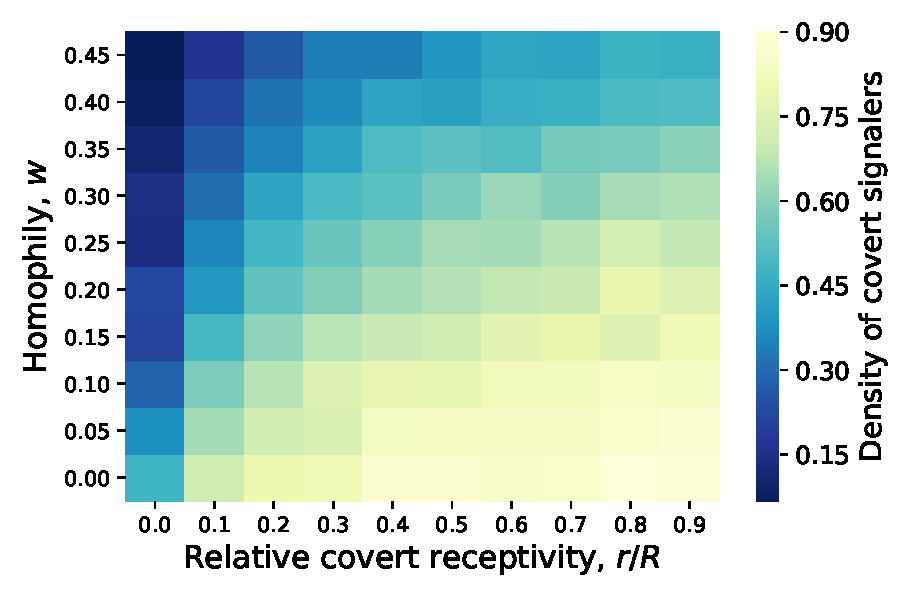
\includegraphics[width=0.8\textwidth]{Figures/covertDensityVsReceptivityHomophily.pdf}
  \caption{Density of covert signalers at $t=100$, final timestep recorded
    in this preliminary experiment.}
  \label{fig:receptivityHomophilyHeatmap}
\end{figure}

\subsection*{Density of covert signalers vs. disliking penalty $d=\delta$ and homophily, $w$}

Here we co-vary the disliking penalties, which we set equal ($d=\delta$), and
homophily, $w$. The bonus payoff for two interacting agents where at least one
likes the other is set to $s=0.25$. The payoff structure is as follows

\begin{table}[h]
  \centering
  \begin{tabular}{rl}
   Attitude combo. & Payoff \\
   \toprule
    Like/like & $1 + s$ \\
    Like/neutral & $1 + s$ \\
    Neutral/neutral & 1 \\
    Like/dislike & $1 + s - d$ \\
    Dislike/neutral & $1 - d$ \\
    Dislike/dislike & $1 - d - \delta$
  \end{tabular}
\end{table}

Specifically, we vary $d=\delta \in \{0.0, 0.05, 0.1, \ldots, 0.45\}
As in the above experiment, we set $w \in \{0.0, 0.5, \ldots, 0.45\}$.
In this experiment we ran the simulations to 200 timesteps 
(Figure~\ref{fig:dislikingHomophilySeries}).

\begin{figure}[H]
  \centering
  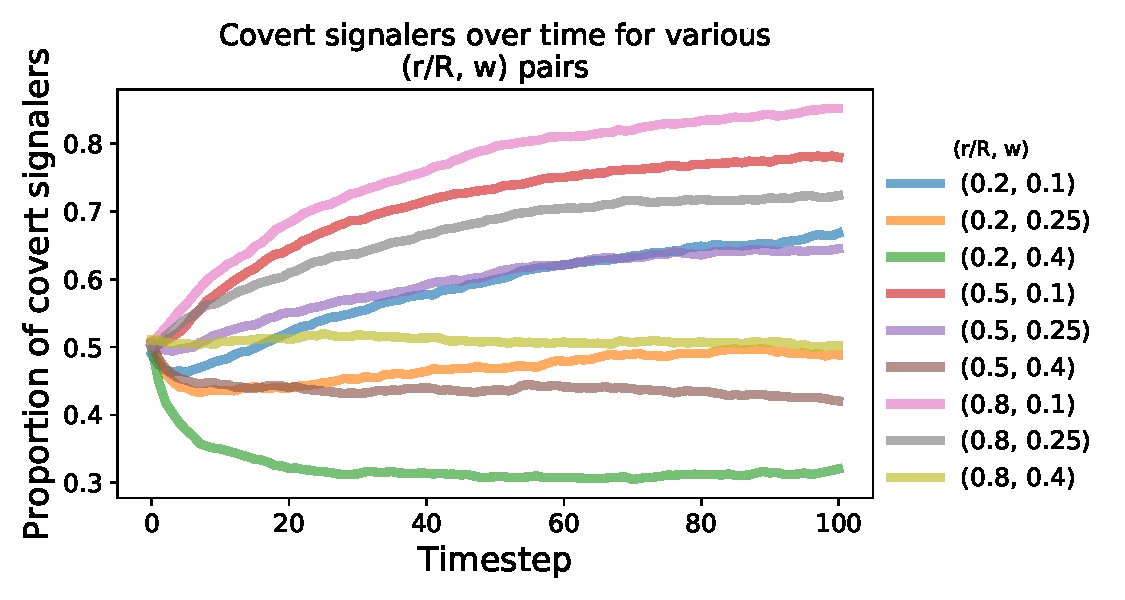
\includegraphics[width=0.8\textwidth]{Figures/exampleMidrangeSeries.pdf}
  \caption{Timeseries of nine combinations of $d=\delta$ and $w$.}
  \label{fig:dislikingHomophilySeries}
\end{figure}

\begin{figure}[H]
  \centering
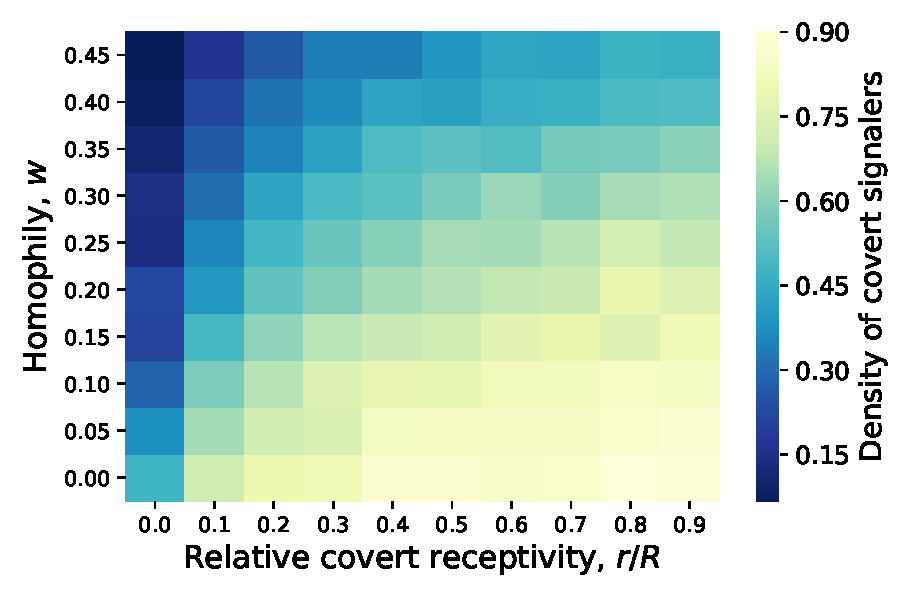
\includegraphics[width=0.8\textwidth]{Figures/covertDensityVsReceptivityHomophily.pdf}
  \caption{Density of covert signalers at $t=100$, final timestep recorded
    in this preliminary experiment.}
  \label{fig:dislikingHomophilyHeatmap}
\end{figure}


\section*{Discussion}

These preliminary experiments and results are based on one major finding from
ECS that covert signaling is maintained when overt signalers do not have
too large an advantage in the free choice context. ``This requires that
assortment with liked individuals not be too accurate,'' which corresponds to
small $w$ in this ABM version. ``The accuracy of assortment is influenced
by the reception probabilities of both signal types, $R$ and $r$'' (see p.
4 in ECS). Our preliminary results find the same trend with our ABM.


% \bibliographystyle{apacite}

% \setlength{\bibleftmargin}{.125in}
% \setlength{\bibindent}{-\bibleftmargin}

% \bibliography{/Users/mt/workspace/papers/library.bib}

\end{document}
